\documentclass{article}
\usepackage{tikz}
\usetikzlibrary{automata, positioning}
\begin{document}
	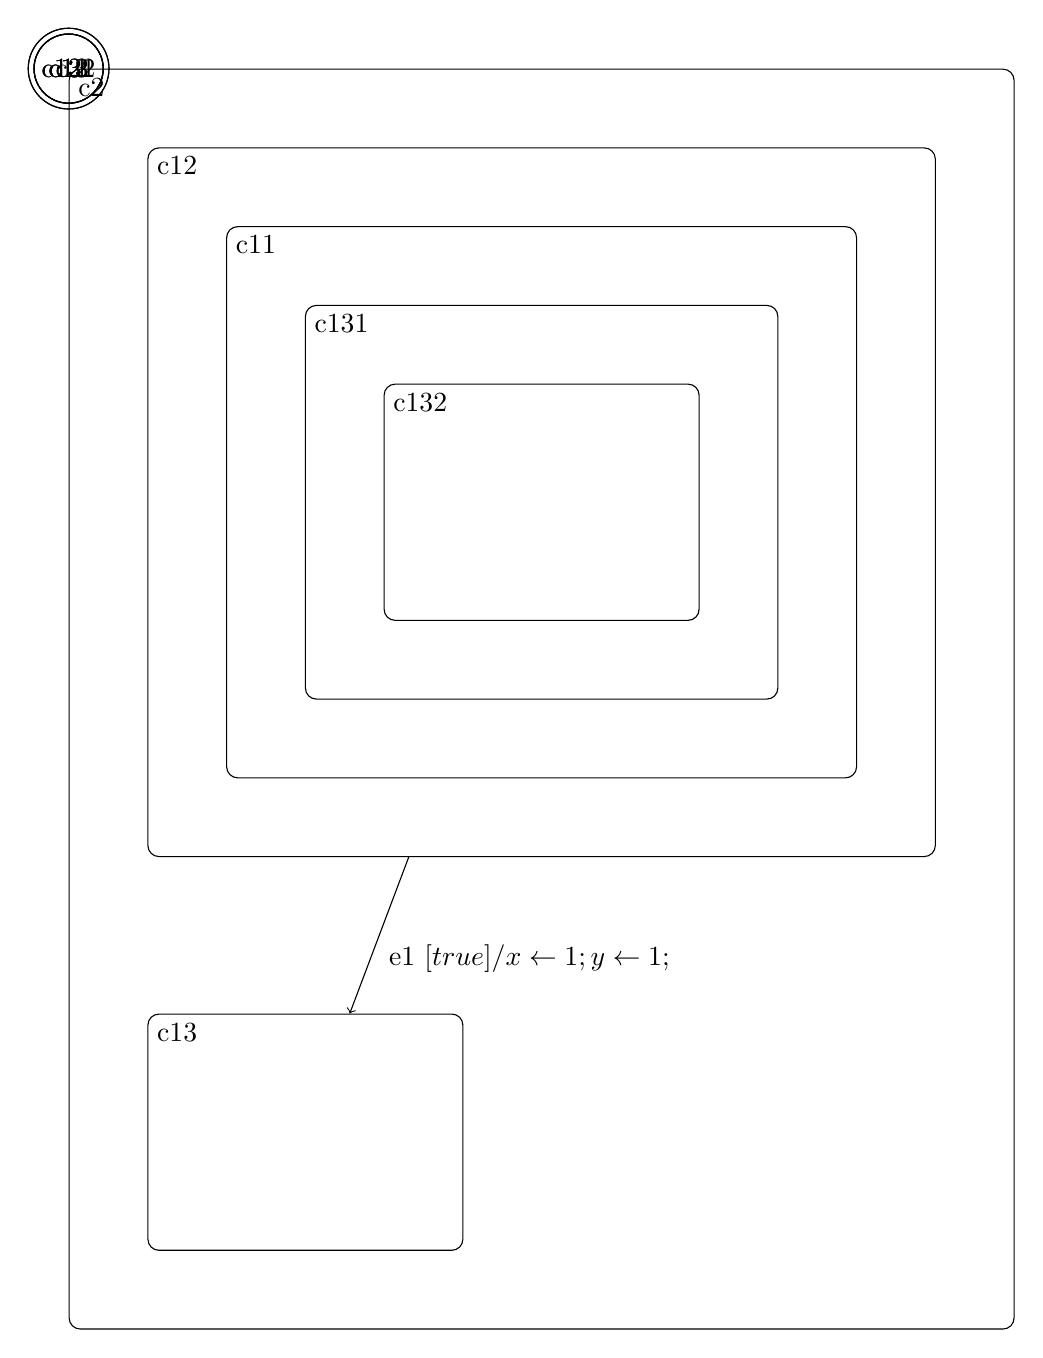
\begin{tikzpicture}[node distance=3cm, auto]
		\node[state] (c2) {c2};
		\node[draw, rectangle, rounded corners, minimum width=12cm, minimum height=16cm, anchor=north west, label={[anchor=north west] north west:c2}] (c2) at (0, 0) {};
		\node[state] (c2_c12) {c12};
		\node[draw, rectangle, rounded corners, minimum width=10cm, minimum height=9cm, anchor=north west, label={[anchor=north west] north west:c12}] (c2_c12) at (1, -1) {};
		\node[state] (c2_c12_c11) {c11};
		\node[draw, rectangle, rounded corners, minimum width=8cm, minimum height=7cm, anchor=north west, label={[anchor=north west] north west:c11}] (c2_c12_c11) at (2, -2) {};
		\node[state] (c2_c12_c11_c131) {c131};
		\node[draw, rectangle, rounded corners, minimum width=6cm, minimum height=5cm, anchor=north west, label={[anchor=north west] north west:c131}] (c2_c12_c11_c131) at (3, -3) {};
		\node[state] (c2_c12_c11_c131_c132) {c132};
		\node[draw, rectangle, rounded corners, minimum width=4cm, minimum height=3cm, anchor=north west, label={[anchor=north west] north west:c132}] (c2_c12_c11_c131_c132) at (4, -4) {};
		\node[state] (c2_c13) {c13};
		\node[draw, rectangle, rounded corners, minimum width=4cm, minimum height=3cm, anchor=north west, label={[anchor=north west] north west:c13}] (c2_c13) at (1, -12) {};
		\draw[->] (c2_c12) edge node  {e1 {$[true]  / x \leftarrow 1; y \leftarrow 1;$}} (c2_c13);
	\end{tikzpicture}
\end{document}
